%\section{Tensor Factorization}   \label{sec:tf}

\section{Multivariate Factorization Model} \label{sec:tf}
A given sensor node may contain multiple sensor types and thus is capable of sensing various aspects of the environment (e.g.\ temperature and humidity) at the same time.
These attributes can potentially be correlated, and being able to take advantage of such correlation would result in better imputation quality.
This section proposes two models, the Multivariate (S)TR-MF and Temporally-Regularized Tensor Factorization (TR-TF), to leverage multivariate correlation for missing data recovery.

\subsection{Multivariate (S)TR-MF} %\label{subsec:Multivariate_TRMF}
In (S)TR-MF, as we normally have much longer time-steps than the number of sensors, the latent matrix $\mathbf{P}$ is much larger than $\mathbf{Q}$, and therefore being able to learn a faithful representation of latent factors in the temporal-dimension is critical. 

Assuming there are two types of sensors in one node: temperature and humidity. Then, using (S)TR-MF we can obtain $\mathbf{P}_{tem}$ and $\mathbf{Q}_{tem}$ from temperature matrix $\mathbf{R}_{tem}$, and get $\mathbf{P}_{hum}$ and $\mathbf{Q}_{hum}$ from humidity matrix $\mathbf{R}_{hum}$. These two $\mathbf{P}$s are identical in size, and it is not hard to imagine that they should be correlated because row factors $\mathbf{p}_m$ in both matrices represents the factors of time step $m$. Therefore, it might be beneficial if we can use both sides of information to learn a unified and better $\mathbf{P}$.
This observation motivates us to design the Multivariate (S)TR-MF.

In Multivariate (S)TR-MF, $\mathbf{R}$ represents the horizontal concatenation of the temperature matrix $\mathbf{R}_{tem}$ and humidity matrix $\mathbf{R}_{hum}$
\begin{equation*} \mathbf{R} = \begin{bmatrix}\mathbf{R}_{tem} & \mathbf{R}_{hum} \end{bmatrix}, \end{equation*}
which allows the temperature model and humidity model to share the common $\mathbf{P}$ matrix, so they merge the similar factors and communicate the observed information with each other. Note that the $\mathbf{Q}_{tem}$ and $\mathbf{Q}_{hum}$ matrix in the (S)TR-MF model remain independent in the new $\mathbf{Q}$ in multivariate (S)TR-MF.

The learning process of multivariate (S)TR-MF is very similar to that of (S)TR-MF: the objective function and the optimization process remains the same. Yet, there are some important differences: 
Firstly, for each row (time step), we need two bias terms: one for temperature readings and the other for humidity readings as they naturally are biased differently. Furthermore, $\mathbf{R}_{tem}$ and $\mathbf{R}_{hum}$ of $\mathbf{R}$ must be normalized independently with their own means and variances. 

 
\subsection{Temporally-Regularized Tensor Factorization Model} \label{sec:tensordecomp}

One main concern for the multivariate (S)TR-MF model is that it does not fully exploit the mutual-dependency between the multiple sensor signals in one node. For instance, we did not specify which column in $\mathbf{R}_{tem}$ corresponds to which column in $\mathbf{R}_{hum}$ as coming from the same node. Therefore, here we propose a more complex tensor model to capture such relationship. 

Tensor can be regarded as a high-dimensional matrix, and is usually exploited to represent multi-dimensional data. The previously introduced TR-MF can model only 2-dimensional correlations such as the sensor/time-step readings. With a 3rd-order tensor, we can add one more dimension into the model (e.g. sensor1/sensor2/time-step or sensor/location/time-step). In order to deal with such high-dimensional data structure, mathematicians have proposed the tensor-decomposition methods to capture its latent factors. 

Tensor decomposition is a multi-dimensional extension of Singular Value Decomposition (SVD). Similar to SVD, Tensor Decomposition methods assume a fully occupied matrix $\mathbf{R}$, while such assumption is not as valid for data imputation purpose as for dimension reduction purpose.
%Treating $\mathbf{R}$ as a dense tensor with missing entries being assume to be 0.
%It would make predict missing value failed.
In the followings, we will first introduce the tensor decomposition models and then describe how we modify one of them into a tensor factorization model for missing data recovery. 

 
\subsubsection{Tensor Decomposition}
Here we introduce two tensor decomposition models in Figure \ref{fig:tf:tuckcanon}. The Tucker decomposition model was first introduced in 1963~\cite{tucker1963implications}, which factorizes a higher-order tensor into a core tensor $\mathbf{S}$ and one factor matrix for each dimension.
A $M\times N \times C $ tensor $\mathbf{T}$ can be decomposed as:

\begin{equation*}
\mathbf{T}=\sum\limits_{i=1}^{I}\sum\limits_{j=1}^{J}\sum\limits_{k=1}^{K}\mathbf{S}_{ijk}\mathbf{p}_i\otimes \mathbf{q}_j\otimes \mathbf{w}_k
\end{equation*}
or for each component,
\begin{equation*}
\mathbf{T}_{mnc}=\sum\limits_{i=1}^{I}\sum\limits_{j=1}^{J}\sum\limits_{k=1}^{K}\mathbf{S}_{ijk}\mathbf{P}_{m i}\mathbf{Q}_{n j}\mathbf{W}_{c k}
\end{equation*}
where the vectors $\mathbf{p}_i$, $\mathbf{q}_j$, and $\mathbf{w}_k$ are the columns of matrices $\mathbf{P}$, $\mathbf{Q}$ and $\mathbf{W}$ respectively, which are the factor matrices and usually orthogonal.
%They can be thought of as the principal components in each order.
%There are several algorithms for calculating Tucker decompositions.
%For data compression, the Tucker decomposition usually assumes that $I\le M$, $J \le N $ and $K \le C$.

%\subsubsection{Canonical Decomposition}

Tucker decomposition is computationally expensive, and researchers have proposed a more efficient Decomposition called Canonical Decomposition~\cite{carroll1970analysis}, which factorizes a tensor into a sum of $K$ rank-one tensors.
Canonical Decomposition~(CD) is the special case of the Tucker decomposition when $\mathbf{S}$ is super-diagonal.
Formally, The Canonical Decomposition of $\mathbf{T}$ is
\begin{equation*}
\mathbf{T}=\sum\limits_{k=1}^{K}\mathbf{x}_k\otimes \mathbf{y}_k\otimes \mathbf{z}_k
\end{equation*}
or
\begin{equation*}
\mathbf{T}_{mnc}=\sum\limits_{k=1}^{K}\mathbf{X}_{m k} \mathbf{Y}_{n k} \mathbf{Z}_{c k}
\end{equation*}
$\mathbf{x}_i$,$\mathbf{y}_i$ and $\mathbf{z}_i$ are a column of matrices $\mathbf{X}$, $\mathbf{Y}$ and $\mathbf{Z}$, which are the factor matrices, and $K$ is the number of columns. 

\begin{figure}[h] 
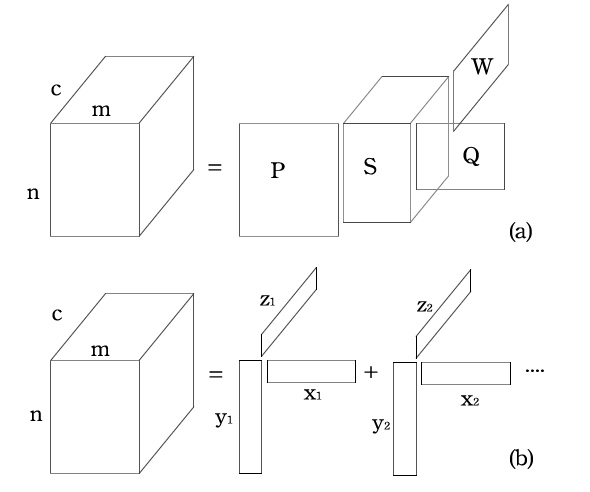
\includegraphics[width=5cm]{tf.jpg} 
\caption{ (a) the Tucker Decomposition (TD) model (b) the Canonical Decomposition model, a special case of the TD model. In sensor networks, the three dimension can be nominal features such as node id, time step index.} 
\label{fig:tf:tuckcanon} 
\end{figure}

\subsubsection{Tensor Factorization for Data Imputation} \label{sec:tfmissing}
%\subsubsection{Objective function}

Existing Tensor Decomposition models require a dense tensor, which is unsuitable for missing data estimation with a decent missing rate. 
Therefore, we introduce an $N$-order Tensor Factorization (TF) model for missing data estimation. Although tensor factorization has been studied for a while and enjoys certain level of success in building context-aware recommender systems~\cite{karatzoglou2010multiverse,rendle2010pairwise}, we have not yet seen any proposal to leverage such techniques for WSN data imputation.

Similar to TR-MF, TR-TF learns the temporal correlation given the sparsity of data with the capability to take additional information such as spatial correlation and heterogeneous sensor readings into consideration.
Consider each reading as a three-dimensional tensor element (e.g. the temperature reading of a sensor given certain time-stamp and certain humidity reading) in $R$, a Tensor can be described as :

\begin{equation*}
\mathbf{T} := F_1 \times  F_2 \times F_3 \rightarrow \mathbf{R} 
\end{equation*}

Tensor factorization model decomposes the reading tensors T into three features, one of them represents the temporal dimension, the rest can represent sensor nodes, sensor node coordinates, heterogeneous sensor readings, etc. In the experiments, we implemented a 3rd-order tensor model and choose the sensor nodes as well as the multivariate sensor readings as the remaining two dimensions.

In contrast to the conventional tensor decomposition, the factorization model we proposed aims at learning the latent factors $\mathbf{P}$,  $\mathbf{Q}$, $\mathbf{W}$ of the three dimensions $F_1, F_2, F_3$.
To avoid over-fitting and to reduce the complexity of prediction, our model borrows the idea of Canonical Decomposition rather than Tucker decomposition. Note that the time complexity for making prediction is only $O(K)$, where $K$ is the factor size of $\mathbf{P}$, $\mathbf{Q}$ and $\mathbf{W}$. Thus, the complexity is independent of the rank of the tensor, which is a favorable property because we can freely add new dimensions into the model without concerning about the efficiency.

Similar to the TR-MF model, we also add bias terms to each dimension into the TF model. The prediction function is:
\begin{equation*}
\begin{aligned}
\mathbf{\hat{T}}_{mnc}=\mu_m+\mu_n+\mu_c + \mathbf{p}_m \otimes \mathbf{q}_n\otimes \mathbf{w}_c
\\=\mu_m+\mu_n+\mu_c+\sum\limits_{k=1}^{K}\mathbf{P}_{m k} \mathbf{Q}_{n k} \mathbf{W}_{c k}
\end{aligned}
\end{equation*}
To learn the latent factors $\mathbf{P}$, $\mathbf{Q}$ and $\mathbf{W}$, we use the loss function :
\begin{equation*}
L(\mathbf{\hat{T}},\mathbf{T})=\frac{1}{\|\mathbf{D}\|_1} \sum\limits_{t\in \mathbf{D}}  l(\hat{t},t)
\end{equation*}
where $\|\mathbf{D}\|$ indicates the size of the observed readings.
$l$ is a point-wise loss function penalizing the distance between estimate and observation.
ideally $l$ should be as close to the eventual evaluation metrics (e.g. least square error in our implementation) as possible.

Simply minimizing a loss function in TF is prone to over-fitting. Here we add regularization terms based on the $L_2$ norm to ensure that the model complexity does not grow without bound to avoid over-fitting.
Similar to our TR-MF model, we also add the time regularization terms into our model.
Finally, the objective function of tensor factorization becomes :\\
\begin{equation*}
\begin{aligned}
&\sum\limits_{m, n, c} l( \hat{\mathbf{T}}_{mnc}, \mathbf{T}_{mnc} )+\beta_1\|\mathbf{p}_{\beta}\|^2+\beta_2\|\mathbf{q}_n\|^2+\beta_3\|\mathbf{w}_c\|^2+\beta_4\|\mu_m\|^2\\
&+\beta_5\|\mu_n\|^2+\beta_6\|\mu_c\|^2+\frac{1}{2}\gamma_1\sum(\mu_m-\mu_{m+1})^2+(\mu_m-\mu_{m-1})^2
\\&
+\frac{1}{2}\gamma_2\sum(\mathbf{p}_m-\mathbf{p}_{m+1})^2+(\mathbf{p}_m-\mathbf{p}_{m-1})^2
\end{aligned}
\end{equation*}

%\begin{algorithm}[h]
%  \caption{Temporally-Regularized Tensor Factorization}
%  \label{alg::conjugateGradient}
%  \textbf{Parameter:} $\beta_1,\beta_2, \beta_3, \beta_4, \beta_5, \beta_6, \gamma_1, \gamma_2, \eta, K$
%  \textbf{Input:} training set, validation set
%  \begin{algorithmic}[1]
%    \State Normalize the training set as $\mathcal{D}$
%    \State Initialize $\mu_m, \mu_n, \mu_c, \mathbf{p}_m, \mathbf{q}_n, \mathbf{w}_c $ for all $m, n, c$
%    \Repeat
%      \For {each observed readings $t$ in $\mathcal{D}$}
%     	 \State Update $\mu_m, \mu_n, \mu_c, \mathbf{p}_m, \mathbf{q}_n, \mathbf{w}_c$ 
%      \EndFor
%     \State Update $\mu_m, \mathbf{p}_m$ for all $m$ by temporal regularization
%    \Until stopping criterion is met
%    \State Output the model for testing set prediction 
%  \end{algorithmic}
%\end{algorithm}

\subsubsection{Optimization}
Minimizing the above objective function can be done using many different strategies.
For efficiency and scalability, we suggest Stochastic Gradient Descent~(SGD) method.
We need to compute the gradients of the objective function with respect to each individual component in the model.
Focusing on an observed reading data t = $T_{mnc} $, the update rules are:
\begin{equation*}
\begin{aligned}
&{\mathbf{p}_m}^\prime={\mathbf{p}_m}+\eta(e*\mathbf{q}_n \mathbf{w}_c - \beta_1 \mathbf{p}_m)
\\&{\mathbf{q}_n}^\prime={\mathbf{q}_n}+\eta(e*\mathbf{p}_m \mathbf{w}_c - \beta_2 \mathbf{q}_n)
\\&{\mathbf{w}_c}^\prime={\mathbf{w}_c}+\eta(e*\mathbf{p}_m \mathbf{q}_n - \beta_3 \mathbf{w}_c)
\\&{\mu_m}^\prime=\mu_m+\eta(e-\beta_4\mu_m)
\\&{\mu_n}^\prime=\mu_n+\eta(e-\beta_5\mu_n)
\\&{\mu_c}^\prime=\mu_c+\eta(e-\beta_6\mu_c)
\end{aligned}
\end{equation*}
where $e=t-\hat{t}$. After a round of updating, we then adjust the parameters according to temporal regularization :
\begin{equation*}
\begin{aligned}
&{\mathbf{p}_m}^\prime={\mathbf{p}_m}+\eta\gamma_1(\mathbf{p}_{m+1}-\mathbf{p}_m+\mathbf{p}_{m-1}-\mathbf{p}_m)
\\&{\mu_m}^\prime=\mu_m+\eta\gamma_2(\mu_{m+1}-\mu_m+\mu_{m-1}-\mu_m)
\end{aligned}
\end{equation*}
%The Temporally-Regularized Tensor Factorization is summarized in Procedure \ref{alg::conjugateGradient}, which is not hard to implement since it accesses only one row of $\mathbf{P}$, $\mathbf{Q}$, $\mathbf{W}$ at a time.

TF applies similar normalization and stopping criterion trick as shown in Section \ref{sec:mf}.
Empirically, one can achieve reasonable performance by imposing the following constraints on the parameter learning:  
\begin{equation*}
\beta_1=\beta_2=\beta_3=\beta_4=\beta_5=\beta_6, \gamma_1=\gamma_2.
\end{equation*}
